\subsection{Initial Constellation Tests} \label{sec:initial_constel}
During preliminary testing, a Molniya and Geosynchronous orbit were simulated. The results ruled them out as practical orbit options, restricting the bulk of study to LEO satellite constellations.
\subsubsection{Molniya Orbit}
A highly inclined molniya orbit was tested with orbital configuration such that the apogee\footnote{Point at which the satellite is farthest from the Earth. For more detail on Molniya orbits See \cite{wertz1999space}} of the orbit occured over the LAX-Heathrow and LAX-Narita flight paths. The ground track of this orbit is shown in Figure \ref{fig:molniya}. It was observed that the satellite would `hang' for long periods of time over the apogee potentially allowing for a longer coverage time. Initial tests yielded a minimum received isotropic power of -162.0 dBW. This was more than 100 times weaker than the worst signal of -140.5 dBW from the set of tested LEO constellations. 

\begin{figure}[H]
	\centering
	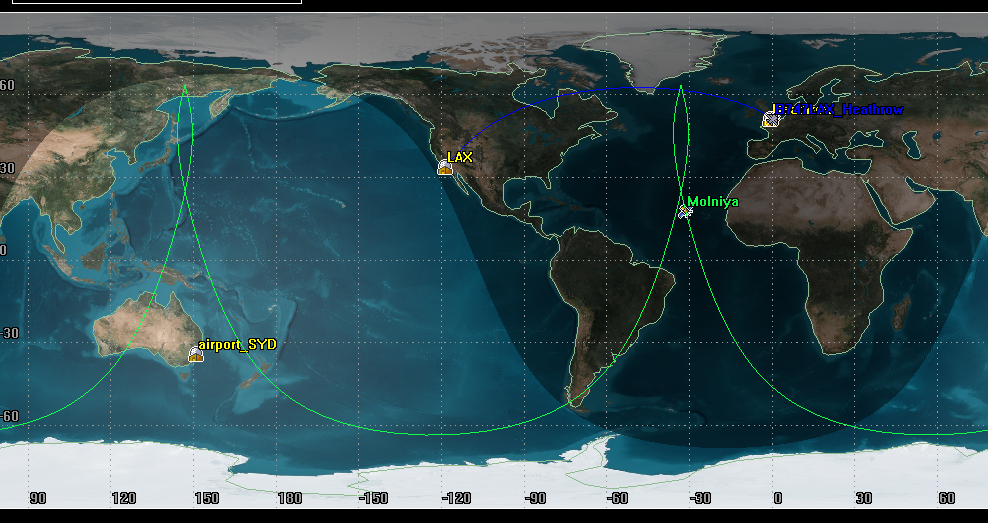
\includegraphics[scale = 0.50]{Pictures/molniya.png}
	
	\caption{Ground track of the tested Molniya orbit}
	\label{fig:molniya}
\end{figure} 

The access times for the LAX-Heathrow flight were evaluated by adding the additional constraint of having a minimum received isotropic power of at least 150.5 dBW (10 times weaker than the worst LEO constellation). This produced a coverage gap fraction of 0.992 \%, meaning that the flight would spend more than 99\% of the time not being able to communicate with an overhead satellite. This result and the poor signal performance resulted in the family of Molniya orbits being ruled out for further analysis.


\subsubsection{Geosynchronous}
A geosynchronous orbit\footnote{See \cite{wertz1999space} for full definition of geosynchronous} was tested with an inclination of 60 degrees and suborbital longitude of -30 degrees in order to place the ground track above the LAX-Heathrow flight. The ground track is given in Figure \ref{fig:geosynch}. The minimum received RX power ranged between -160.3 dBW in the best case and -161.7 dBW in the worse case. This orbit was then dismissed because of the poor performing worst case signal when compared with LEO constellations. 

\begin{figure}[H]
	\centering
	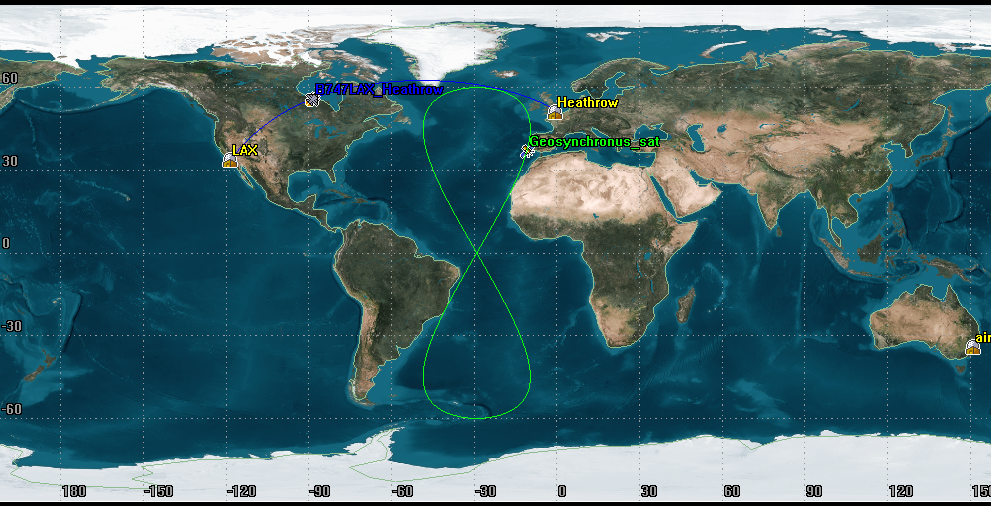
\includegraphics[scale = 0.55]{Pictures/geosynch.png}
	
	\caption{Ground track of the tested Geosynchronous orbit}
	\label{fig:geosynch}
\end{figure} 
